

\section{Homotopical behavior of desingularization}
\label{sec:behavior}

In this section, we display examples of the behavior of desingularization. Specifically, we display the results of desingularizing a few models of spheres. In \cref{sec:inverse}, we explain that the two-fold Kan subdivision $Sd^2$ performed before desingularization ensures that the homotopy type is not altered. This is analogous to Thomason's situation \cite{Th80}. Note that performing the Kan subdivision once before desingularization is not enough.

Forming the colimit of a diagram in $nsSet$ can be done by forgetting that the involved simplicial sets are non-singular, forming the colimit in $sSet$ instead, and finally applying desingularization.

Consider some of the usual models for spheres. It is not hard to realize that
\[D(\Delta [n]/\partial \Delta [n])\cong \Delta [0]\]
for every $n>0$. Not much harder is it to see that
\[DSd(\Delta [n]/\partial \Delta [n])\cong \Delta [1]\]
for every $n>1$. Thus in these cases, desingularization does not preserve homotopy type. Note that the case $n=1$ is special as $Sd(\Delta [1]/\partial \Delta [1])$ is two copies of $\Delta [1]$ glued together along their boundaries. Hence, this simplicial set is already non-singular. So desingularization trivially preserves homotopy type in this case.

The $2$-sphere can be modeled by $X=Sd^2(\Delta [2]/\partial \Delta [2])$. This is because the Kan subdivision preserves colimits \cite[Cor.~4.2.11]{FP90} and degreewise injective maps \cite[Cor.~4.2.9]{FP90}. Hence, the simplicial set $Sd^2(\partial \Delta [2])$ can be considered the boundary of $Sd^2(\Delta [2])$ and the simplicial set $X$ is the result of collapsing this boundary. \cref{fig:ch1_Desing_doublysubd_2simpl} is meant to indicate that $DX$ is the suspension of a $1$-sphere, modelled by a 12-gon, which we have formulated as \cref{prop:double_subdivision_sphere_low_dimension}. In other words, desingularization preserves the homotopy type in this case. One might attribute the behavior to properties of the inclusion
\[Sd^2(\partial \Delta [2])\to Sd^2(\Delta [2])\]
of the boundary. \cref{def:strom}, \cref{cor:two-fold_subdivision_strom} and \cref{lem:Pushout_along_strom_homotopically_wellbehaved} will make this claim precise. The intuition is that the two-fold subdivision creates a sufficiently nice neighborhood around the boundary.

Here we transfer Thomason's insights \cite[Prop.~4.3]{Th80}, which most likely come from regular neighborhood theory, to our setting. Regular neighborhood theory is treated in the sources \cite[§3]{RS72} and \cite[§II]{Hu69}.

The functor $DSd$ takes the instance
\[d_{\Delta [2]/\partial \Delta [2]}:Sd(\Delta [2]/\partial \Delta [2])\xrightarrow{\sim } \Delta [2]/\partial \Delta [2]\]
of the last vertex map, which is in general a weak equivalence, to a map whose source is a model of the $2$-sphere and whose target is contractible. Hence, we get the following result.
\begin{lemma}\label{lem:non-existence_result_mod_str}
Let $sSet$ have the standard model structure due to Quillen. There is no model structure on $nsSet$ such that $DSd$ is a left Quillen functor.
\end{lemma}
\begin{proof}
Any simplicial set is cofibrant in the standard model structure on $sSet$ due to Quillen. This is because the cofibrations are precisely the degreewise injective maps. See Proposition 3.2.2. in Hovey's book \cite{Ho99} for a reference.

\begin{figure}
\centering
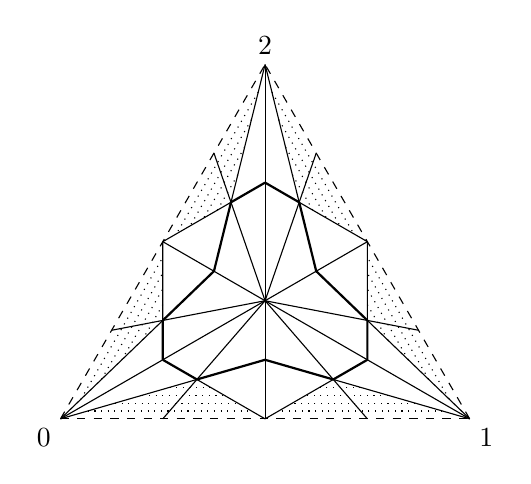
\begin{tikzpicture}

% Vertices of a triangle
\coordinate (2) at (90:3cm);
\coordinate (0) at (210:3cm);
\coordinate (1) at (-30:3cm);

% Nodes to mark vertices of a triangle
\node [above] at (2) {2};
\node [below left] at (0) {0};
\node [below right] at (1) {1};

% Draw line between the vertices 0,1 and 2 and name the midpoints
\draw [dashed] (0.north east)--(2.south) coordinate[midway](02);
\draw [dashed] (0.north east)--(1.north west) coordinate[midway](01);
\draw [dashed] (1.north west)--(2.south) coordinate[midway](12);

% Barycenter, could also be found by means of the intersection library of tikz
\coordinate (012) at (barycentric cs:0=1,1=1,2=1);

% Draws lines from vertices of original triangle to barycentre of original triangle and...
\draw (0.north east)--(012) coordinate[midway](0<012);
\draw (1.north west)--(012) coordinate[midway](1<012);
\draw (2.south)--(012) coordinate[midway](2<012);
\draw (01)--(012) coordinate[midway](01<012);
\draw (12)--(012) coordinate[midway](12<012);
\draw (02)--(012) coordinate[midway](02<012);

% Subdivide each of the six new 2-simplices. To highlight the structure of the desingularized simplicial set we make certain lines thicker
\coordinate (0<01<012) at (barycentric cs:0=1,01=1,012=1);
\coordinate (0<01) at (barycentric cs:0=0.5,01=0.5);
\foreach \x in {(0),(0<01),(01),(012)}
	\draw (0<01<012)--\x;
\foreach \x in {(0<012),(01<012)}
	\draw [thick] (0<01<012)--\x;

\coordinate (1<01<012) at (barycentric cs:1=1,01=1,012=1);
\coordinate (1<01) at (barycentric cs:1=0.5,01=0.5);
\foreach \x in {(1),(1<01),(01),(012)}
	\draw (1<01<012)--\x;
\foreach \x in {(01<012),(1<012)}
	\draw [thick] (1<01<012)--\x;

\coordinate (1<12<012) at (barycentric cs:1=1,12=1,012=1);
\coordinate (1<12) at (barycentric cs:1=0.5,12=0.5);
\foreach \x in {(1),(1<12),(12),(012)}
	\draw (1<12<012)--\x;
\foreach \x in {(12<012),(1<012)}
	\draw [thick] (1<12<012)--\x;

\coordinate (2<12<012) at (barycentric cs:2=1,12=1,012=1);
\coordinate (2<12) at (barycentric cs:2=0.5,12=0.5);
\foreach \x in {(2),(2<12),(12),(012)}
	\draw (2<12<012)--\x;
\foreach \x in {(12<012),(2<012)}
	\draw [thick] (2<12<012)--\x;
	
\coordinate (2<02<012) at (barycentric cs:2=1,02=1,012=1);
\coordinate (2<02) at (barycentric cs:2=0.5,02=0.5);
\foreach \x in {(2),(2<02),(02),(012)}
	\draw (2<02<012)--\x;
\foreach \x in {(02<012),(2<012)}
	\draw [thick] (2<02<012)--\x;
	
\coordinate (0<02<012) at (barycentric cs:0=1,02=1,012=1);
\coordinate (0<02) at (barycentric cs:0=0.5,02=0.5);
\foreach \x in {(0),(0<02),(02),(012)}
	\draw (0<02<012)--\x;
\foreach \x in {(02<012),(0<012)}
	\draw [thick] (0<02<012)--\x;

% Effect of desingularizing doubly subdivided 2-simplex with collapsed boundary. We make these lines dotted.
\foreach \x in {0.2,0.4,0.6,0.8}
	\draw [dotted] (barycentric cs:0=\x,0<01<012=1-\x)--(barycentric cs:01=\x,0<01<012=1-\x);

\foreach \x in {0.2,0.4,0.6,0.8}
	\draw [dotted] (barycentric cs:1=\x,1<01<012=1-\x)--(barycentric cs:01=\x,1<01<012=1-\x);

\foreach \x in {0.2,0.4,0.6,0.8}
	\draw [dotted] (barycentric cs:1=\x,1<12<012=1-\x)--(barycentric cs:12=\x,1<12<012=1-\x);

\foreach \x in {0.2,0.4,0.6,0.8}
	\draw [dotted] (barycentric cs:2=\x,2<12<012=1-\x)--(barycentric cs:12=\x,2<12<012=1-\x);

\foreach \x in {0.2,0.4,0.6,0.8}
	\draw [dotted] (barycentric cs:2=\x,2<02<012=1-\x)--(barycentric cs:02=\x,2<02<012=1-\x);

\foreach \x in {0.2,0.4,0.6,0.8}
	\draw [dotted] (barycentric cs:0=\x,0<02<012=1-\x)--(barycentric cs:02=\x,0<02<012=1-\x);
\end{tikzpicture}
\caption{Desingularizing the double subdivision of the standard $2$-simplex with collapsed boundary.}
\label{fig:ch1_Desing_doublysubd_2simpl}
\end{figure}


By Ken Brown's lemma \cite[Lem.~1.1.12, p.~6]{Ho99} a left Quillen functor takes each weak equivalence between cofibrant objects to a weak equivalence. However, $DSd(d_{\Delta [2]/\partial \Delta [2]})$ is not a weak equivalence. Thus $DSd$ is not a left Quillen functor.
\end{proof}
\noindent Moreover, the diagram
\begin{displaymath}
\xymatrix{
DSd^2(\Delta [2]) \ar[d]^\sim & DSd^2(\partial \Delta [2]) \ar[l] \ar[d]^\sim \ar[r] & DSd^2(\Delta [0]) \ar[d]^\sim \\
DSd(\Delta [2]) & DSd(\partial \Delta [2]) \ar[l] \ar[r] & DSd(\Delta [0])
}
\end{displaymath}
indicates that the map $DSd(\partial \Delta [2])\to DSd(\Delta [2])$ is most likely a non-candidate for a cofibration whenever $nsSet$ is a left proper model category. \cref{lem:non-candidate_cofibration} below justifies this educated guess.

We recall the axiom of propriety, which is desirable in a model category. Consider a commutative square
\begin{displaymath}
 \xymatrix{
 X \ar[d]_i \ar[r]^f & Z \ar[d]^j \\
 Y \ar[r]_g & W
 }
\end{displaymath}
in some category. If the square is cartesian, then we say that $f$ is the \textbf{base change of $g$ along $j$}. If it is cocartesian, then we say that $g$ is the \textbf{cobase change of $f$ along $i$}.
\begin{definition}
Consider a model category. We say that the model category is \textbf{right proper} if weak equivalences are preserved under taking base change along fibrations. Consider a model category. We say that the model category is \textbf{left proper} if weak equivalences are preserved under taking cobase change along cofibrations. If a model category is both right proper and left proper, then we say that it is \textbf{proper}.
\end{definition}
\noindent Note that $sSet$ with the standard model structure is proper \cite[Thm.~13.1.13, p.~242]{Hi03}.

There is a glueing lemma that says that if we have a commutative diagram
\begin{displaymath}
\xymatrix{
B \ar[d]^\sim & A \ar[l] \ar[d]^\sim \ar[r] & C \ar[d]^\sim \\
Y & X \ar[l] \ar[r] & Z
}
\end{displaymath}
in a left proper model category such that at least one map in each row is a cofibration and such that all the vertical maps are weak equivalences, then the canonical map
\[B\sqcup _AC\xrightarrow{\sim } Y\sqcup _XZ\]
of pushouts is a weak equivalence. A reference for the dual of this result is Proposition 13.3.9 in Hirschhorn's book \cite[pp.~246--247]{Hi03}. Note that a more common glueing lemma demands that $A\to B$ and $X\to Y$ be cofibrations and not simply that at least one map in each row be a cofibration.

The former of the two versions of the glueing lemma yields the following result.
\begin{lemma}\label{lem:non-candidate_cofibration}
Assume that $nsSet$ is given a model structure such that it is a left proper model category whose weak equivalences are those maps $f$ such that $\lvert Uf\rvert$ is a (weak) homotopy equivalence. Then neither of the two maps
\[DSd(\partial \Delta [2])\to DSd(\Delta [2])\]
and
\[DSd(\partial \Delta [2])\to DSd(\Delta [0])\]
is a cofibration or neither of the two maps
\[DSd^2(\partial \Delta [2])\to DSd^2(\Delta [2])\]
and
\[DSd^2(\partial \Delta [2])\to DSd^2(\Delta [0])\]
is a cofibration.
\end{lemma}
\noindent \cref{lem:non-candidate_cofibration} justifies the educated guess that $DSd(\partial \Delta [2])\to DSd(\Delta [2])$ is most likely not a cofibration, though it does not imply that the map is not a cofibration.

Before we can state the nature of these properties we need a few definitions. Let $\varepsilon ^n_j:[0]\to [n]$ be the \textbf{vertex operator} given by $0\mapsto j$. Usually, we omit the upper index.
\begin{definition}
Let $X$ be a simplicial set, and $A$ a simplicial subset. We say that $A$ is \textbf{full} if it has the property that any simplex of $X$ is a simplex of $A$ provided its vertices
are in $A$.
\end{definition}
\begin{definition}
Suppose $X$ a simplicial set. Let $A$ be a full simplicial subset of $X$. We say that $A$ is an \textbf{eden (resp. abyss)} in $X$ if it has the property that any $1$-simplex $x$ of $X$ whose first (resp. zeroth) vertex $x\varepsilon _1$ (resp. $x\varepsilon _0$) is in $A$, is itself is a simplex of $A$.
\end{definition}
\noindent We wish to compare the new notions with analogous notions in the $Cat$, partly because the intuition is more readily available in $Cat$ than in $sSet$.

Consider the notions of sieve and cosieve.
\begin{definition}
Suppose $\mathscr{C}$ a small category. Let $\mathscr{D}$ be a subcategory of $\mathscr{C}$. We will say that $\mathscr{D}$ is a \textbf{(co)sieve} in $\mathscr{C}$ if whenever we have a morphism $c\to c'$ whose target (source) is an object of $\mathscr{D}$, then the morphism is itself a morphism of $\mathscr{D}$.
\end{definition}
\noindent Intuitively, a sieve is a place to which there is no entry and a cosieve is a place from which there is no escape. The notion of sieve corresponds to the notion of eden and the notion of cosieve corresponds to the notion of abyss. In $PoSet$, the notion of sieve is equivalent to the notion of ideal when a poset is thought of as a set equipped with a reflexive, antisymmetric and transitive binary operation.

Note the following relationship between the notions of sieve and eden and between cosieve and abyss.
\begin{lemma}\label{lem:nerve_of_(co)sieve}
The nerve of a sieve (resp. cosieve) is an eden (resp. abyss).
\end{lemma}
\noindent Furthermore, note the following characterization.
\begin{lemma}\label{lem:(co)sieve_characterization_elementary}
A simplicial subset $A$ of a simplicial set $X$ is an eden in $X$ if and only if any simplex whose last vertex is in $A$ is also a simplex of $A$. Similarly, the simplicial subset $A$ is an abyss in $X$ if and only if any simplex whose zeroth vertex is in $A$ is also a simplex of $A$.
\end{lemma}
\noindent \cref{lem:(co)sieve_characterization_categorical} below provides another characterization that is more useful.

Performing desingularization is messy in general. However, there are useful situations in which the process is predictable. Such as when one desingularizes a quotient $X/A$ of a non-singular simplicial set $X$ by an eden $A$. \cref{prop:desingularizing_after_collapsing_elysium} will make this precise. Understanding the behavior of $D$ towards quotients of the kind we mentioned is vital to our discussion of the properties of Str\o m maps.

The new notions are of the following categorical nature.
\begin{lemma}\label{lem:(co)sieve_characterization_categorical}
A simplicial subset $A$ of a simplicial set $X$ is an eden (resp. abyss) if and only if there is a map
$\chi :X\rightarrow \Delta [1]$ such that the square
\begin{displaymath}
 \xymatrix{
 A \ar[d] \ar[r] & \Delta [0] \ar[d]^{N\varepsilon _0\; (\textrm{resp.} \; N\varepsilon _1)} \\
 X \ar[r]_(.45)\chi & \Delta [1]
 }
\end{displaymath}
is cartesian. Here,
\[\varepsilon _0:[0]\to [1]\; (\textrm{resp.} \; \varepsilon _1:[0]\to [1])\]
is the vertex operator given by
\[0\mapsto 0\; (\textrm{resp.} \; 0\mapsto 1).\]
We refer to $\chi$ as the \textbf{characteristic map of $A$ as an eden (resp. abyss) in $B$}.
\end{lemma}
\noindent The proof of this lemma is straight-forward, and is left out.

Part of the interest in the notion of eden is that the Kan subdivision creates edens from arbitrary simplicial subsets, which we state as \cref{lemma_subdivision_creates_left_sieve} below. First, we remind the reader how to define the Kan subdivision.

Consider a simplicial set $X$ and the poset $X^\sharp$ of non-degenerate simplices. There is a morphism $y\to x$ from $y$ to $x$ if $y$ is a face of $x$. The operation of taking a simplicial set $X$ to $X^\sharp$ defines a functor $(-)^\sharp :sSet\to PoSet$.  A map $f:X\to Y$ induces the map $f^\sharp :X^\sharp \to Y^\sharp$ given by sending $x$ to the non-degenerate part $f(x)^\sharp$ of $f(x)$.
\begin{lemma}\label{lem:sharp_creates_sieves}
Let $X$ be a simplicial set and let $A$ be a simplicial subset of $X$. Then $A^\sharp$ is a sieve in $X^\sharp$.
\end{lemma}
\noindent This observation will be used in the proof of \cref{lem:Barratt_nerve_of_inclusion_of_non-sing_is_strom} below.
\begin{definition}\label{def:Barratt_nerve}
We refer to the endofunctor of simplicial sets defined on objects by $BX=N(X^\sharp )$ as the \textbf{Barratt nerve}.
\end{definition}
\noindent Note that this terminology is not standard. We follow \cite[Def.~2.2.3, p.~35]{WJR13}, but Fritsch and Piccinini call $B$ the \emph{star functor} \cite[Exercise~4.6.33,~p.~219]{FP90}. The \textbf{Kan subdivision} is the left Kan extension of $B$ along the Yoneda embedding $\Upsilon :\Delta \to sSet$. Loosely, the Kan subdivision is the best way to adapt \emph{barycentric subdivision} to simplicial sets.

We can elaborate the previous paragraph. The \textbf{simplex category} of $X$, denoted $\Delta \downarrow X$, is the small category whose objects are the representing maps $\bar{x}$ of simplices of $X$ and whose morphisms $\bar{y} \to \bar{x}$ are the commutative diagrams
\begin{displaymath}
\xymatrix@=1em{
\Delta [m] \ar[dr]_{\bar{y} } \ar[rr]^{\alpha } && \Delta [n] \ar[ld]^{\bar{x} } \\
& X
}
\end{displaymath}
whenever $y$ is of degree $m$ and $x$ is of degree $n$. Note that we simplify the notation slightly by writing $\alpha$ in place of $N\alpha$, where $\alpha :[m]\to [n]$ must by definition be an operator such that $y=x\alpha$.

One can view the Kan subdivision of $X$ as
\[Sd\; X\cong colim(B\circ \Upsilon _X),\]
where $\Upsilon _X:\Delta \downarrow X\to sSet$ is the composite of Yoneda embedding $[n]\xmapsto{\Upsilon } \Delta [n]$ with the forgetful functor $(x,n)\mapsto [n]$. A simplicial map $f:X\to Y$ gives rise to a functor $\Delta \downarrow f$ such that $\Upsilon _X=\Upsilon _Y\circ \Delta \downarrow f$. In particular, the identity is a natural transformation
\[\Upsilon _X\Rightarrow\Upsilon _Y\circ \Delta \downarrow f.\]
From this arises the map $Sd(f):Sd\, X\to Sd\, Y$ in an intuitive way.

Combining the diagram $B\circ \Upsilon _Y$ with its colimit $Sd\, Y$ gives rise to a cocone on $B\circ \Upsilon _Y\circ \Delta \downarrow f$ with apex $Sd\, Y$ and thus a map
\[colim(B\circ \Upsilon _Y\circ \Delta \downarrow f)\to Sd\, Y.\]
The identity natural transformation $\Upsilon _X\Rightarrow\Upsilon _Y\circ \Delta \downarrow f$ gives rise to a natural transformation
\[B\circ \Upsilon _X\Rightarrow B\circ \Upsilon _Y\circ \Delta \downarrow f,\]
which must be the identity as well. Thus the map above with target $Sd\, Y$ can be considered to have $Sd\, X$ as its source. The map itself is denoted $Sd(f)$.

We can take the viewpoint that
\[X\cong colim(\Upsilon X)\]
\cite[Lem.~4.2.1~(ii),~p.~141]{FP90}. In other words, the cocone $\Upsilon _X\Rightarrow \underline{X}$, meaning the natural transformation from $\Upsilon _X$ to the constant diagram that takes every object to $X$, is universal. Combining this with $B$ yields a cocone $B\circ \Upsilon _X\Rightarrow \underline{BX}$ with apex $BX$. It gives rise to a canonical map $b_X:Sd\, X\to BX$.
\begin{lemma}
\label{lem:properties_of_b_X}
The canonical map $b_X:Sd\, X\to BX$ is natural, degreewise surjective and an isomorphism if and only if $X$ is non-singular.
\end{lemma}
\begin{proof}
The naturality is automatic when $b_X$ comes from the viewpoint that $Sd$ is the left Kan extension of $B$ along the Yoneda embedding. See \cite[Lem.~2.2.10, p.~38]{WJR13} for the statement and proof that $b_X$ is degreewise surjective. See \cite[Lem.~2.2.11, p.~38]{WJR13} for the statement and proof that $b_X$ is an isomorphism if and only if $X$ is non-singular.
\end{proof}
\noindent We will make use of the comparison map $b_X$ in the proof of the crucial result stated as \cref{cor:two-fold_subdivision_strom}.

As promised, the Kan subdivision creates sieves.
\begin{lemma}\label{lemma_subdivision_creates_left_sieve}
Let $X$ be a simplicial set and $A$ a simplicial subset. Then $\textrm{Sd} \, A$ is an eden in $\textrm{Sd} \, X$.
\end{lemma}
\begin{proof}[Proof of Lemma~\ref{lemma_subdivision_creates_left_sieve}]
Let $i:A\to X$ be the inclusion. We will construct a natural transformation
\[B\circ \Upsilon _X\xRightarrow{\psi } \underline{\Delta [1]},\]
which gives rise to a map $\chi :\textrm{Sd} \,X\to \Delta [1]$. Next, we will verify that $Sd\, A\to \Delta [0]$ is a base change of $\chi$ along $N\varepsilon _0$.

Given an object $\bar{x} :\Delta [n]\to X$ of $\Delta \downarrow X$ we define
\[\psi _{\bar{x} }:B(\Delta [n])\to \Delta [1]\]
by letting it be the nerve of $\Delta [n]^\sharp \to [1]$ given by sending an object $\mu$ of $\Delta [n]^\sharp$ to $0$ if $x\mu$ is a simplex of $A$, and to $1$ otherwise.

We verify that the triangle
\begin{displaymath}
\xymatrix@=1em{
 B(\Delta [m]) \ar[dd]_{B(N\alpha )} \ar[dr]^{\psi _{\bar{y} }} \\
 & \Delta [1] \\
 B(\Delta [n]) \ar[ur]_{\psi _{\bar{x} }}
 }
\end{displaymath}
commutes whenever $\alpha$ is such that $y=x\alpha$. To this end, take some face operator $\mu \in \Delta [m]^\sharp$ with target $[m]$. The order-preserving function $(N\alpha )^\sharp$ sends $\mu$ to the face operator $(\alpha \mu )^\sharp$. We can write $y\mu$ as a degeneracy
\[y\mu =x\alpha \mu =x(\alpha \mu )^\sharp (\alpha \mu )^\flat\]
of $x(\alpha \mu )^\sharp$. This means that $y\mu$ is a simplex of $A$ if and only if $x(\alpha \mu )^\sharp$ is a simplex of $A$. In other words, the underlying triangle of posets commutes. Thus $\psi _{\bar{x} }$ is natural, as claimed.

As a result of the previous paragraph we now have the composite natural transformation
\[B\circ \Upsilon _X\Rightarrow \underline{Sd\, X} \Rightarrow \underline{\Delta [1]} \]
between functors $\Delta \downarrow X\to sSet$. This composite induces a composite of natural transformations between functors $\Delta \downarrow A\to sSet$, through precomposition with $\Delta \downarrow i$. By the design of $\psi$, the latter factors through $N\varepsilon _0:\Delta [0]\to \Delta [1]$. This way we obtain a commutative square
\begin{displaymath}
\xymatrix{
B\circ \Upsilon X\circ \Delta \downarrow i \ar@{=>}[d] \ar@{==>}[r] & \underline{\Delta [0]} \ar@{=>}[d]^{\underline{N\varepsilon _0} } \\
\underline{Sd\, X} \ar@{=>}[r] & \underline{\Delta [1]}
}
\end{displaymath}
of natural transformations and thus a candidate $\chi :Sd\, X\to \Delta [1]$ for a characteristic map. It remains to verify that, if given a solid arrow commutative diagram
\begin{displaymath}
 \xymatrix{
 Z \ar@/^2pc/[drr] \ar@{-->}[dr] \ar@/_2pc/[ddr]_f \\
 & Sd\, A \ar[d]_{Sd(i)} \ar[r] & \Delta [0] \ar[d]^{N\varepsilon _0} \\
 & Sd\, X \ar[r]_(.45)\chi & \Delta [1]
 }
\end{displaymath}
then there exists a dashed map $Z\to Sd\, A$ that makes the whole diagram commute. There is at most one such map $Z\to Sd\, A$ as $Sd(i)$ is degreewise injective. Because $\Delta [0]$ is a terminal object it is enough to verify that $f$ factors through $Sd(i)$. As $Sd(i)$ is degreewise injective it suffices to verify that the image of $f$ is contained in the image of $Sd(i)$.

Suppose $z$ a $q$-simplex of $Z$. By the commutativity of the solid arrow diagram, we get that
\[N\varepsilon _0 \circ g(z)=\chi \circ f(z).\]
We argue that $f(z)\in Sd(X)_q$ is in the image of $Sd(i)_q$.

The simplex $f(z)$ is the image of some element $\varphi :[q]\to \Delta [n]^\sharp \in \Upsilon _X(\bar{x} )$ such that $\varphi (q)$ is the identity. Write $\varphi _j=\varphi (j)$ for $0\leq j\leq q$. Because $\chi \circ f(z)$ is in the image of $N\varepsilon _0$, it follows that $x\varphi _j$ is a simplex of $A$ for each $j$ with $0\leq j\leq q$. In particular, the simplex $x\varphi _q$ is a simplex of $A$. The face operator $\varphi _q$ is the identity, so $x=x\varphi _q$ is itself a simplex of $A$. Thus $f(z)$ is in the image of $Sd(i)$.
\end{proof}
\noindent Now we know that a simplicial subset of a simplicial set can always be turned into an eden by applying the Kan subdivision.

The following term is central.
\begin{definition}\label{def:strom}
A map $k:A\to B$ in $nsSet$ is referred to as a \textbf{Strøm map} if the following conditions hold.
\begin{enumerate}
\item{The map $k$ is a degreewise injective map whose image is an eden in $B$.}
\item{There is an abyss $W$ in $B$ such that $k$ can be factored as $i:A\to W$ followed by the inclusion $j:W\to B$.}
\item{The map $i$ is a section of some map $r:W\to A$.}
\item{The simplicial set $W$ is deformable rel $A$ to $A$ in $W$, namely there exists a simplicial homotopy $\epsilon :W\times \Delta [1]\to W$ such that the diagrams
\begin{displaymath}
\xymatrix{
W \ar[d]_{i_0} \ar[dr]^{ir} && A\times \Delta [1] \ar[dd]_{pr_1} \ar[r]^{i\times1} & W\times \Delta [1] \ar[dd]_{\epsilon } \\
W\times \Delta [1] \ar[r]^\epsilon & W  \\
W \ar[u]^{i_1} \ar[ur]_1 && A \ar[r]^i & W
}
\end{displaymath}
commute.}
\end{enumerate}
\end{definition}
\noindent Notice that the image of $k$ is an eden in $W$.

The class of Str\o m maps is not a category as a composite of Str\o m maps is not necessarily a Str\o m map. This is because the two simplicial homotopies as described in \cref{def:strom} that come with two composable Str\o m maps do not necessarily give rise to a new simplicial homotopy that satisfies the fourth condition of \cref{def:strom}. Compare with class of pseudo-Dwyer maps \cite{Ci99}, which does form a subcategory of $Cat$.

A bit of history may be of interest to the reader. The class of Str\o m maps fills the same role in establishing $nsSet$ as a model category (Quillen equivalent to $sSet$) as the class of \emph{Dwyer maps} in Thomason's paper \cite{Th80}, where $Cat$ is established as a model category (Quillen equivalent to $sSet$). However, a mistake in Thomason's proof intially left the axiom of propriety unproven.

After having established the model structure, Thomason asserted that the Dwyer maps were closed under retracts. As any cofibration was a retract of a Dwyer map, Thomason concluded that any cofibration was a Dwyer map. Therefore, as the nerve functor $N$ took a cocartesian square in $Cat$ with at least one leg Dwyer to a homotopy cocartesian square in $sSet$, it would follow that $Cat$ is left proper. However, the Dwyer maps are not closed under retracts \cite{Ci99}.

This mistake was not a fatal mistake, as it turned out. Cisinski was able to correct the proof of the axiom of propriety by weakening the definition of the term Dwyer map and thus creating a new notion that he gave the ad hoc name \emph{pseudo-Dwyer map}. Perhaps the new notion is better referred to under the name \emph{Cisinski map}. The notion of Cisinski map may have been borrowed from A. Str\o m as it is an analogue to one of his characterizations \cite[Thm.~2~(ii), p.~12]{St66} of the cofibrations for the Str\o m model structure on topological spaces \cite{St72}. It is the model structure whose weak equivalences are the homotopy equivalences and whose fibrations are the Hurewicz fibrations.

Cisinski argues that $N$ takes a cocartesian square in $Cat$ with at least one leg Cisinski to a homotopy cocartesian square in $sSet$ \cite{Ci99}. Thus Thomason's argument that $Cat$ is left proper goes through when Dwyer maps are replaced by Cisinski maps. Cisinski takes the correction one step further and points out that Cisinski maps are closed under cobase change and under taking compositions of $\aleph _0$-sequences \cite{Ci99}. Indeed, Raptis points out that both Dwyer maps and Cisinski maps are closed under (transfinite) compositions \cite[Prop.~2.4.~(a),~p.~216]{Ra10}. Thus, using Thomason's original technique, Thomason's model structure on $Cat$ can be established by means of the term Cisinski map alone, although the notion of Dwyer map plays a role in Thomason's discussion regarding cofibrant objects \cite[Lemma 5.6.~(4),p.~323]{Th80}.

Crucially, the sets $DSd^2(I)$ and $DSd^2(J)$ are contained in the class of Str\o m maps, as we will now argue.
\begin{lemma}\label{lem:Barratt_nerve_of_inclusion_of_non-sing_is_strom}
Let $k:A\to X$ be an inclusion of a simplicial subset $A$ into a non-singular simplicial set $X$. If $A$ is an eden in $X$, then $B(k)$ is a Str\o m map.
\end{lemma}
\begin{proof}
Let $W$ be the subposet of $X^\sharp$ whose objects are precisely the non-degenerate simplices of $X$ that have a face in $A$. As $A$ is an eden it follows that there is a greatest face in $A$ of any given element of $W$. If $w\in W$, we let $r(w)$ denote this unique face. Because $X$ is non-singular it follows that $r(w)$ is non-degenerate, hence an object of $A^\sharp$. Moreover, we get a functor $r:W\to A^\sharp$. It is a retraction of the corestriction $i$ of $k^\sharp :A^\sharp \to X^\sharp$ to $W$.

By \cref{lem:sharp_creates_sieves}, the functor $(-)^\sharp$ creates sieves. Therefore, we get that $A^\sharp$ is a sieve in $X^\sharp$. By the definition of $W$ it follows that it is a cosieve in $X^\sharp$. Furthermore, \cref{lem:nerve_of_(co)sieve} says that $BA=N(A^\sharp )$ is an eden in $BX=N(X^\sharp )$ and that $NW$ is an abyss in $BX$.

If $w\in W$, then there is a morphism $ir(w)\to w$ by the definition of $r$. The rest of the argument is standard. Namely, because $W$ is a poset it is true that $ir(w)\to w$ is automatically natural. This natural morphism from $ir$ to the identity can be viewed as a functor $W\times [1]\to W$, which in turn gives rise to a simplicial homotopy $NW\times \Delta [1]\to NW$ from $Ni\circ Nr$ to the identity as $N$ preserves limits and in particular products. The simplicial homotopy is stationary on $N(A^\sharp )$ because it is identified with the nerve of $W\times [1]\to W$, which is stationary on $A^\sharp$ in an intuitive, analogous sense. This concludes the proof that $B(k)$ is a Str\o m map.
\end{proof}
\begin{corollary}\label{cor:two-fold_subdivision_strom}
Let $Y$ be a simplicial set such that $Sd\, Y$ is non-singular and let $X$ be a simplicial subset of $Y$. If $k:X\to Y$ is the inclusion, then $Sd^2(k)$ is Str\o m.
\end{corollary}
\begin{proof}
According to \cref{lemma_subdivision_creates_left_sieve}, we have that $Sd\, X$ is an eden in $Sd\, Y$. By \cref{lem:Barratt_nerve_of_inclusion_of_non-sing_is_strom} we now know that $BSd(k)$ is Str\o m. The naturality of $b_{Sd\, X}$ means that we can identify $BSd(k)$ with $Sd^2(k)$ via the diagram
\begin{displaymath}
\xymatrix{
Sd^2\, X \ar[d]_{Sd(Sd(k))} \ar[r]^{b_{Sd\, X}}_\cong & BSd\, X \ar[d]^{B(Sd(k))} \\
Sd^2\, Y \ar[r]_{b_{Sd\, Y}}^\cong & BSd\, Y
}
\end{displaymath}
as $Sd\, X$ and $Sd\, Y$ are non-singular. This is because the natural map from the Kan subdivision to the Barratt nerve is an isomorphism when the original simplicial set is non-singular \cite[Lem.~2.2.11, p.~38]{WJR13}. Hence, the map $Sd^2(k)$ is a Str\o m map.
\end{proof}
\noindent In particular, if $k$ in \cref{cor:two-fold_subdivision_strom} is one of the inclusions $\partial \Delta [n]\to \Delta [n]$ or one of the inclusions $\Lambda ^j[n]\to \Delta [n]$, then we see that $Sd^2(k)$ is a Str\o m map.


